\documentclass[letterpaper, 11pt]{article}
%\setcounter{secnumdepth}{0}
\usepackage{fontspec}
\usepackage{ctable}
\defaultfontfeatures{Ligatures=TeX}
\usepackage[small,sf,bf]{titlesec}
\usepackage{amsmath}
\usepackage{amssymb}
\usepackage[empty]{fullpage}
\setlength{\parskip}{\medskipamount}
\usepackage{nopageno}

\usepackage{caption}
\captionsetup[table]{skip=10pt}

\usepackage{rotating}
\usepackage{rotfloat}

\usepackage{listings}
%\newfontfamily\Consolas{DejaVu Sans Mono}
%\lstset{basicstyle=\footnotesize\Consolas}

\setmainfont{CMU Serif}

\raggedbottom
\raggedright

\providecommand{\e}[1]{\ensuremath{\times 10^{#1}}}
\newcolumntype{L}{>{$}l<{$}} % math-mode version of "l" column type
\newcolumntype{C}{>{$}c<{$}} % math-mode version of "c" column type
\newcolumntype{R}{>{$}r<{$}} % math-mode version of "r" column type
%\newcolumntype{C}{ >{\centering\arraybackslash} m{6cm} }
%\newcolumntype{D}{ >{\centering\arraybackslash} m{4.5cm} }

\newcommand{\norm}[1]{\left\lVert #1 \right\rVert}
\newcommand{\vect}[1]{\boldsymbol{#1}}

\makeatletter
\renewcommand*\env@matrix[1][*\c@MaxMatrixCols c]{%
  \hskip -\arraycolsep
  \let\@ifnextchar\new@ifnextchar
  \array{#1}}
\makeatother

\begin{document}

\renewcommand{\arraystretch}{1.1}

\title{Regularization and transformation:\\CSE802 Project}
\author{Jonny Dowdall, James Peterkin II, Eric Alan Wayman}
\date{Submitted May 4, 2018}
\maketitle

\section{Introduction}

\subsection{Motivation}

The fact that the performance of classifiers can be improved through methods that 1) impose some form of regularization on the estimated parameters, or 2) exploit useful transformations of the feature space, suggests that understanding of the intracies and interrelationships between these techniques is an important part of any practitioner's toolbox in the field of pattern recognition and machine learning. Our project seeks to build such an understanding and to test that understanding against the application of the techniques to real-world datasets.

The basic idea of regularization is that when fitted to a particular training data set models may learn the idiosyncracies of that data set (overfitting) and that will be reflected in poorer performance on an unseen test data set compared to the performance of the average of a series of models fit to various training sets. Regularization simulates this procedure by restricting the magnitude of components of the parameter vector, forcing the fitted model to be more ``smooth'' than if the parameter vector were unrestricted. Overfitting can also be addressed through sparsity-encouraging regularization ($\ell_1$ regularization, which increases the ``signal to noise ratio'' by encouraging the parameter coefficients of features that do not contribute to reducing model error to go to zero). 

Underfitting occurs when the model is too simple for the data. Since the models in this project produce linear decision boundaries, this will occur when features are not linearly separable in the original feature space. Transforming the data to a higher-dimensional feature space, in this project demonstrated by the use of the RBF kernel, may allow the data to become linearly separable in that feature space. Through the use of the kernel trick, the model can be fit in the higher-dimensional space through performing calculations in the original feature space, and the resulting decision boundary visualized in the original feature space.

Overfitting can also be addressed through fitting the data using a subset of the training points, and by choosing a linear boundary that separates the data points with as large a ``margin'', or distance from the closest points to the boundary, as possible. Both of these qualities are characteristics of the Support Vector Machine (SVM).

Another classifier, logistic regression, can be used in conjunction with the $\ell_1$ and $\ell_2$ norms for regularization, as well as with transformed data (kernelized logistic regression). The details of all these techniques will be explained in sections to follow.

\subsection{Literature review}

Regularization was first proposed by Tychonoff (Theodoridis 2015, 72) in 1977 (Tychonoff and Arsenin 1977). $\ell_1$ and $\ell_2$ regularization are common techniques described in many machine learning textbooks, for example Murphy 2015.

Logistic regression, the first of the two classifiers that were used in this project, was invented by David Cox in 1958 (Cox 1958).

According to Wikipedia, kernel classifiers were likely first mentioned in the 1960s (Aizerman et al. 1964) and gained widespread attention due to the introduction of the support vector machine (SVM) in the 1990s due to the SVM's competitive performance on tasks such as handwriting recognition. This SVM, which uses the ``kernel trick'' to be described below was invented by Boser et al. in 1992 (Boser et. al 1992).

The usage of kernels with logistic regression is demonstrated in Zhu and Hastie (2002).

The techniques explained and used in this project are widely used in pattern classification (for example see).

\subsection{Problem statement}

To explain how techniques of regularization and data transformation can be used in conjunction with the binary classifers logistic regression and SVM, use this understanding to hypothesize regarding the performance of the various techniques on datasets with differing characteristics, and test these hypotheses on real-world datsets.

On datasets which are linearly separable, we expect 

\section{Approach}

\subsection{Logistic regression with $\ell_1$ and $\ell_2$ regularization}

Logistic regression is a discriminative classifier. It corresponds to a binary classification model:

\begin{equation*}
  p(y | \vect{x}, \vect{w}) = \text{Ber}(y | \text{sigm}(\vect{w}^T\vect{x}))
\end{equation*}

(Murphy 2012, 245) where sigm is the sigmoid function. If the possible values of $y$ are either $-1$ or $+1$, then $p(y = 1) = 1 / (1 + \exp(-\vect{w}^T\vect{x}))$ and $p(y = -1) = 1 / (1 + \exp(\vect{w}^T\vect{x}))$. We minimize the error by maximizing the negative log-likelihood:

\begin{equation*}
  NLL(\vect{w}) = \log(1 + \exp(-y_i \vect{w}^T\vect{x}))
\end{equation*}

(Murphy 2012, 245). There is not a closed-form solution for the MLE of $\vect{w}$, so it must be estimated by an optimization algorithm. However, we must often design constraints to prevent the parameters from overfitting the training data and losing generality.

\subsubsection{The effects of $\ell_1$ and $\ell_2$ regularization}

When the $\ell_2$ regularization term is included, maximizing the NLL function with respect to $\vect{w}$ and $\lambda$ tries to reduce the norm of $\vect{w}$ (the vector of parameters) while at the same time minimizing the error given by the log-likelihood cost function (maximizing the negative of this function). This helps prevent overfitting: by restricting the $\ell_2$ norm of $\vect{w}$, the ``complexity'' of the model is restricted, so it is prevented from ``learning too much about the idiosyncrasies of the specific training data set'' (Theodoridis 2015, 74).

If only a few features contain significant information and there are a large number of features, the ``true'' model generating the data will have the coefficients of most components of $\vect{w}$ equal to zero. Therefore it 

The following figure (Figure 1, taken from Theodoridis 2015, 406, Figure 9.2) shows the relationship between a given component $\theta$ of the parameter vector $\vect{\theta}$ (what we call $\vect{w}$) and its contribution to $\norm{\vect{\theta}}_p$, $|\theta|^p$, for given levels of $p$. For $\ell_p$ norms with $p \geq 1$, components $\theta$ with larger $|\theta|^p$ give a larger contribution to the norm, so assuming for example's sake that two components $\theta_1$ and $\theta_2$ have the same effect on the fit of the model and $|\theta_1|^p > |\theta_2|^p > 1$, the minimization will try to reduce the size of $\theta_1$ more than $\theta_2$. Conversely, for $p > 1$, any $\theta_j$ with $|\theta_j|^p < 1$ will not have its size reduced very much at all, irrespective of the amount to which it contributes to minimizing the error of the model.

\subsubsection{Applying regularization to logistic regression}

$\ell_1$ regularization is achieved by adding the term $\lambda {\norm{\vect{w}}_1}^2$ where $\norm{\vect{w}}_1 = \sum_{i=1}^{c} |\vect{w}_i|$ (Theodoridis 2015, 404), so

\begin{equation*}
  NLL(\vect{w}, \lambda) = \log(1 + \exp(-y_i \vect{w}^T\vect{x})) + \lambda {\norm{\vect{w}}_1}
\end{equation*}


$\ell_2$ regularization is achieved by adding the term $\frac{\lambda}{2} {\norm{w}_2}^2$ to $NLL(\vect{w})$ above, giving

\begin{equation*}
  NLL(\vect{w}, \lambda) = \log(1 + \exp(-y_i \vect{w}^T\vect{x})) + \frac{\lambda}{2} {\norm{\vect{w}}_2}^2
\end{equation*}

However, for $p = 1$, even components $\theta_j$ with $|\theta_j|^1 < 1$ will have the regularization applied to them. Therefore irrespective of the size of a true $\theta_j$, the regularization will force $\theta_j$ to 0 if it does not contribute to minimizing model error.

(The above discussion was based Theodoridis 2015, 406-407)

\begin{figure}[ht!]
\centering
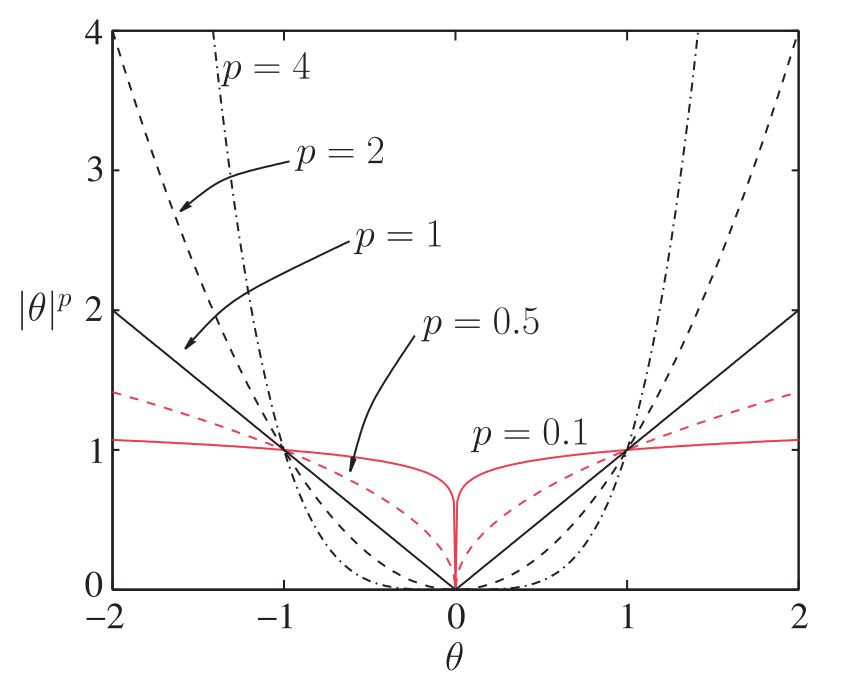
\includegraphics[width=90mm]{figure1.jpg}
\caption{CHANGE THISSS!!!!!!!!! \label{overflow}}
\end{figure}

\subsection{Kernels: linear vs RBF}

Kernels are commonly used to model similarities over pairs of data points. A Mercer kernel is a kernel whose Gram matrix

\begin{equation*}
  \vect{K} = \begin{pmatrix}
    \kappa(\vect{x}_1, \vect{x}_1) & \cdots & \kappa(\vect{x}_1, \vect{x}_N) \\
    & \vdots & \\
    \kappa(\vect{x}_N, \vect{x}_1) & \cdots & \kappa(\vect{x}_N, \vect{x}_N) \\    
  \end{pmatrix}
\end{equation*}

is positive semi-definite for any set of inputs $\{\vect{x}_i\}_{i=1}^N$ (Murphy 2012, 481). For any Mercer kernel there exists a function $\vect{\phi}: \mathcal{X} \rightarrow \mathbb{R}^D$ for which then $K(\vect{x}, \vect{x}^\prime) = \vect{\phi}(\vect{x})^T\vect{\phi}(\vect{x})$. Note that $D$ can be infinite, as explained in the section ``SVM and RBF kernel relationship explanation.''

In this project we use two kernels, linear kernels and the RBF kernel, both of which are Mercer kernels. The kernels will be used in this project as transformations of data to be input to classifiers which produce a linear decision boundary (if transformed data is input to a classifier, the resulting decision boudary will be linear in that transformed space).

Note that usually it is hard to derive the feature vector $\vect{\phi}(\vect{x})$ from a Kernel $\kappa(\vect{x}, \vect{x}^\prime)$, but the reverse is not difficult for a Mercer kernel since $\kappa(\vect{x}, \vect{x}^\prime) = \vect{\phi}(\vect{x})$.

The linear kernel is $\kappa(\vect{x}, \vect{x}^\prime) = \vect{x}^T\vect{x}^\prime$, which corresponds to the case where $\vect{\phi}(\vect{x}) = \vect{x}$, so $\vect{\phi}(\vect{x})$ takes points in $\mathcal{X}$ to $\mathcal{X}$. This kernel is useful in the case where the decision boundary is linear in the original feature space, so transforming them to a higher-dimensional feature space is not necessary (Murphy 2012, 482).

The RBF kernel is defined as follows:

\begin{equation*}
  K(\vect{x}, \vect{x}^\prime) = \exp\left(-\gamma \norm{\vect{x} - \vect{x}^\prime}\right)
\end{equation*}

As noted above, the $D$ in $\vect{\phi}(\vect{x}): \mathcal{X} \rightarrow \mathbb{R}^D$ is infinite in the case of the RBF kernel. To understand the transformation, following Abu-Mostafa et al. (8-37), let $\gamma = 1$ and $\vect{x}$ be a scalar. Then

\begin{align*}
  K(x, x^\prime) & = \exp\left(-\norm{x - x^\prime}^2\right) \\
  & = \exp\left(-(x)^2\right) \cdot \exp\left(2xx^\prime\right) \cdot \exp(-\left(x^\prime\right)^2) \\
  & = \exp\left(-(x)^2\right) \cdot \left(\sum_{k=0}^{\infty} \frac{2^k(x)^k\left(x^\prime\right)^k}{k!}\right) \cdot \exp\left(-\left(x^\prime\right)^2\right)
\end{align*}

Defining

\begin{equation*}
  \vect{\phi}(x) = \exp(-x^2) \cdot \left(1, \sqrt{\frac{2^1}{1!}}x, \sqrt{\frac{2^1}{2!}}x^2, \sqrt{\frac{2^1}{3!}}x^3, \ldots \right)
\end{equation*}

we see that $K(x, x^\prime) = \vect{\phi}(x)^T \vect{\phi}(x)$. The right hand side is an inner product in an infinite-dimensional feature space, which shows that the $D$ in the range of $K$ can be infinite.

\subsubsection{The ``kernel trick''}

If it is difficult to compute $\vect{\phi}(\vect{x})^T \vect{\phi}(\vect{x})$, instead we can compute $K(\vect{x}, \vect{x}^\prime)$ in the original $\mathcal{X}$ space since the results are equal. For the kernels used in this project, this is useful for the RBF kernel, as exact calculation of $\vect{\phi}(\vect{x})^T \vect{\phi}(\vect{x})$ in the range space of $\vect{\phi}$ is impossible. 

\subsection{SVMs}

The SVM is a classifier that incorporates sparsity of data points (as opposed to features) into its loss function (Murphy 2012, 497). SVMs for classification use a loss function called hinge loss, which is of the form $L_\text{hinge}(y, \eta) = \max(0, 1 - y \eta) = (1 - y\eta)_{+}$ where $\eta = f(\vect{x})$ is the ``confidence'' (not necessarily a probability) in choosing label $y = 1$ (Murphy 2012, 499). The objective function is

\begin{equation*}
  \min_{\vect{w}, w_0} \frac{1}{2}{\norm{\vect{w}}_2}^2 + C \sum_{i=1}^{N}(1 - y_i f(\vect{x}_i))_{+}
\end{equation*}

This is non-differentiable, but by introducing slack variables, the minimization problem can be transformed to one solvable by quadratic programming (Murphy 2012, 499).

\subsubsection{Generalization and the large-margin principle}

The minimization problem mentioned in the previous paragram can be obtained through a different approach, namely maximizing the size of the margin $f(\vect{x}) / \norm{\vect{w}}_2$. This approach also depends on the introduction of slack variables which allows the problem to handle certain cases. The resulting objective function is the same as the approach from minimizing the hinge loss function.

The importance of the large-margin is that it helps the model's generalization performance (Theodoridis 2015, 550). An intuitive way to see this is by Figure 2 (this is Figure 14.11 from Murphy 2012, 500).

\subsubsection{Generalization and support vectors}

The solution for the weights for the SVM has the form $\widehat{\vect{w}} = \sum_i \alpha_i \vect{x}_i$ where $\vect{\alpha}$ has many entries equal to 0; the $\vect{x}_i$ corresponding to non-zero $\alpha_i$ are called support vectors. Since the parameter vector for the fitted SVM depends only on a subset of data points, this helps model generalizability (Theodoridis and Koutroumbas 2009, 206).

\begin{figure}[ht!]
\centering
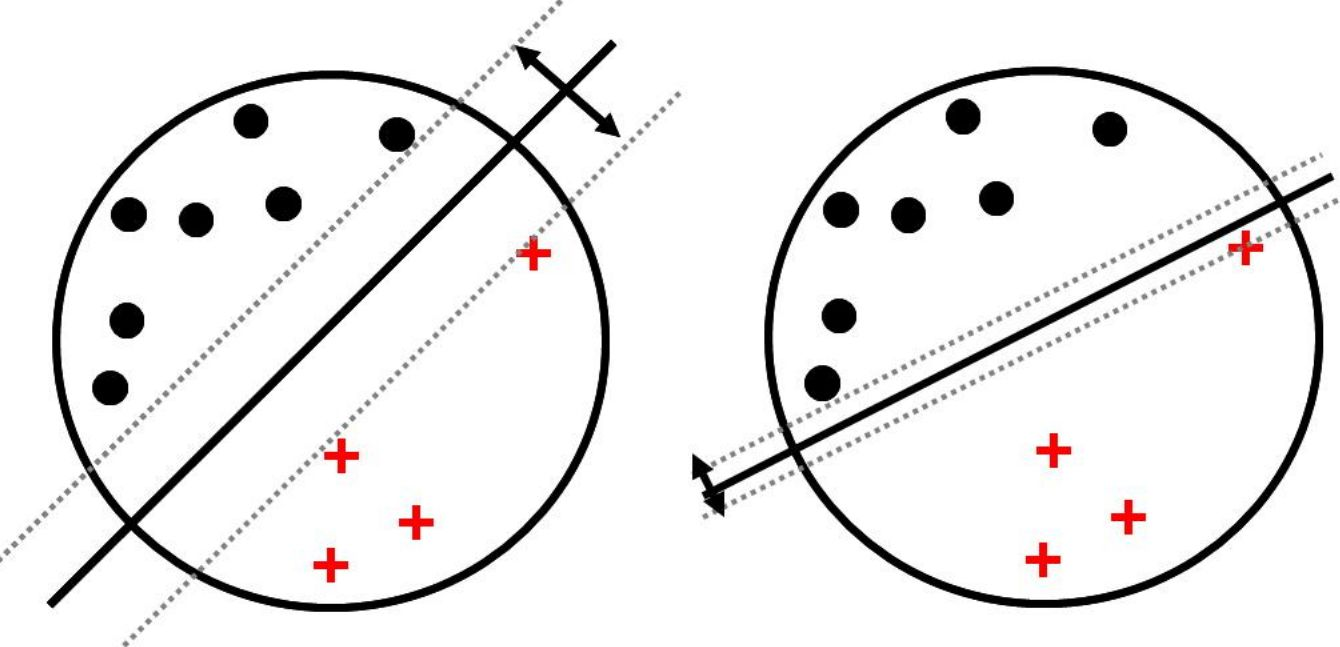
\includegraphics[width=120mm]{largeMarginPrinciple2.jpg}
\caption{A simple caption \label{overflow}}
\end{figure}

The SVM is used in this project with both the linear and RBF kernels.

\subsection{SVM and logistic regression with the RBF kernel: a close relationship}

In this section, we explain the effects of using logistic regression on data that has been transformed with the RBF kernel, and how this relates to the case where an SVM is used with such transformed data.

The optimal $f(\vect{x})$ in fitting an SVM is of the form $f(\vect{x}) = \sum_{i=1}^{n} \alpha_i K(\vect{x}, \vect{x}_i^\prime)$ (Zhu and Hastie 2002, 186). Also since the negative log-likelihood (NLL) for logistic regression has a similar shape to the NLL of the SVM, replacing the NLL of the SVM with the NLL of the logistic regression gives roughly the same solution (Zhu and Hastie 2002, 186). Then for a Mercer kernel, the interpretation of the probability $p(\vect{x})$ (which equals $P(y = 1 | \vect{X} = \vect{x})$, Lin 2002) is

\begin{align*}
  p(\vect{x}) & = \frac{e^{f(\vect{x})}}{1 + e^{f(\vect{x})}} = \frac{1}{1 + \exp({-f(\vect{x})})} & \\
  & = \frac{1}{1 + \exp(-\sum_{i=1}^{n} \alpha_i K(\vect{x}, \vect{x}_i^\prime))} & \text{plugging in the optimal solution} \\
  & = \frac{1}{1 + \exp(-\sum_{i=1}^{n} \alpha_i \vect{\phi}(\vect{x}_i)^T \vect{\phi}(\vect{x}))} & \text{using the kernel trick} \\
  & = \frac{1}{1 + \exp(-\vect{w}^T \vect{\phi}(\vect{x}))} &
\end{align*}

where the last step is by defining $\vect{w} = \sum_{i} \alpha_i \vect{\phi}(\vect{x}_i)$ is the weighted sum of transformed support vectors. The last two steps here were taken from Guestrin (2007). This implies that the kernel trick can be used to run logistic regression on data that has been transformed to an infinite-dimensional feature space using the $\vect{\phi}$ corresponding to the RBF kernel.

\subsection{Summary of model fitting strategies and data transformations}

The following table summarizes the combinations of model fitting strategies and data transformations used in this project. Each column indicates a different model fitting strategy (used in conjunction, of course, with minimizing model error as represented by a loss function), while each row indicates a type of data transformation. Each cell indicates the classifier that was used in conjuction with the fitting strategy and data transformation. Note that the model used for any particular combination is deterministic: in other words, the desired model fitting strategy and data transformation indicate a model choice.

\begin{center}
  \begin{tabular}{l|c|c|c|c|}
         & vanilla & $\ell_1$ & $\ell_2$ & few data pts \& large margin \\
\hline
  linear &         & log reg  & log reg  & SVM \\
\hline
  RBF    & log reg &          &          & SVM \\
\hline
\end{tabular}
\end{center}

\begin{description}
\item[vanilla:] loss function with no regularization term \\
\item[loss + $\ell_1$:] loss function with $\ell_1$ regularization term \\
\item[loss + $\ell_2$:] loss function with $\ell_2$ regularization term
\item[few data pts \& large margin] model attempts to utilize small subset of of training data in parameter estimation, and attempts to maximize size of margin while minimizing error 
\end{description}

\section{Datasets}

\section{Experimental analysis}

\section{Findings}

\section{Summary and future work}

\section{Works cited}

Abu-Mostafa, Malik Magdon-Ismail and Hsuan-Tien Lin. 2012. \emph{Learning with data}, e-Chapter 8 (``Support vector machines'') AMLBook.

Gretton, Arthur et al. 2012. "A Kernel Two-Sample Test." Journal of Machine Learning Research. Vol 13, p. 723-773.

Guestrin, Carlos. 2007. ``Support vector machines.'' Lecture slides for ``Machine Learning – 10701/15781`` at Carnegie Mellon University. 

Hsu, Chih-Wei et al. 2016. "A Practical Guide to Support Vector Classification." Department of Computer Science, National Taiwan University.

Lin, Yi. 2002. ``Support vector machines and the Bayes rule in classification.'' \emph{Data Mining and Knowledge Discovery} (6): 259–275.

Murphy, Kevin. 2012. \emph{Machine learning: a probabilistic perspective}. MIT Press: Cambridge, MA.

Theodoridis, Sergios and Konstantinos Koutroumbas. 2009. \emph{Pattern recognition}. Academic Press: Burlington, MA.

Theodoridis, Sergios. 2015. \emph{Machine learning: a Bayesian and optimization perspective}. Academic Press: London, United Kingdom.

Zhu, Ji and Trevor Hastie. 2004. ``Kernel logistic regression and the import vector machine.'' \emph{Journal of Computational and Graphical Statistics}.  
Volume 14, 2005 - Issue 1.

\section{References cited in literature review}

Aizerman, M. A., Emmanuel M. Braverman and Rozoner, L. I. 1964. "Theoretical foundations of the potential function method in pattern recognition learning". \emph{Automation and Remote Control}. 25: 821–837.

Boser, Bernhard E., Isabelle M. Guyon and Vladimir N. Vapnik. 1992. "A training algorithm for optimal margin classifiers". \emph{Proceedings of the fifth annual workshop on Computational learning theory – COLT '92}. p. 144.

Cox, DR. 1958. "The regression analysis of binary sequences (with discussion)". \emph{J Roy Stat Soc B}. 20: 215–242.

Tychonoff, A.N. and V.Y. Arsenin. \emph{Solution of ill-posed problems}. Winston \& Sons: Washington, 1977.

\end{document}
